

\subsection{Request a new sensor}

\hrule
\hfill
\vspace{0.5cm}
\label{operation:Request a new sensor}

The Technician can request a new sensor.
\begin{description}
\item \textbf{Parameters:} NameSensor,RoomNumber,TechnicianName,Reason
\item \textbf{Precondition:} The system is bootedup and the technician has to be
logged in and be on the technician screen.
\item \textbf{Post-condition:} Updated request sensor table.
\item \textbf{Output messages:}Message with the request pulled to the manager.
\item \textbf{Triggering:}
\begin{enumerate}
\item \textbf{Technician} Complets the diffrent input fields and presses the
button push to the manager.
\begin{figure}[H]
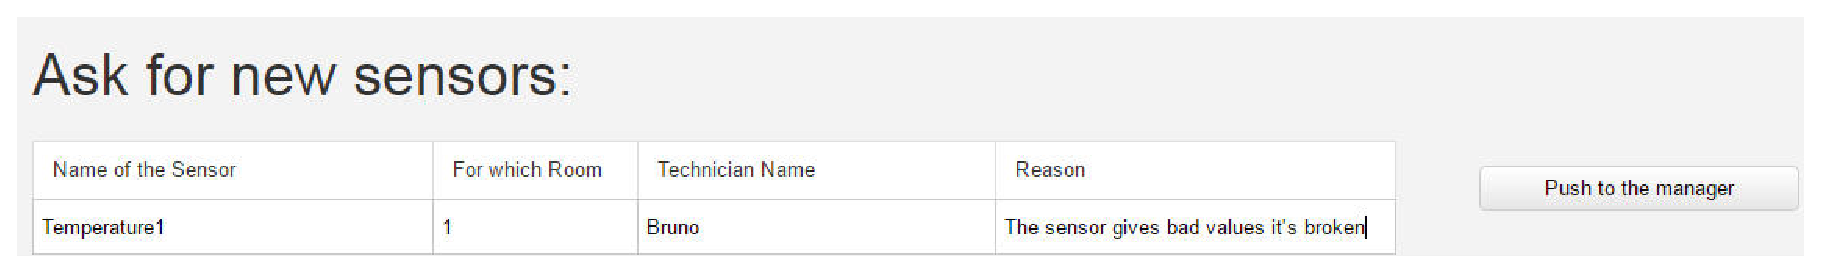
\includegraphics[width=1\textwidth]{images/AskForANewSensor.eps}
\end{figure}
\item System sends the information to the manager by updating the request
sensor table.
\end{enumerate}
\end{description}

\subsubsection{Example of a request of a sensor}
\textbf{Technician} complets the input text field with their given information
that means Name of the Sensor:Temperature1 RoomNumber:1 Technician Name: Bruno
and Reason Sensor Temperature 1 gives wrong information sensor is
damaged.\textbf{System} inserts this information to the manager request sensor
table.
\hfill
\vspace{0.5cm}
\hrule



\subsection{Add a new sensor}

\hrule
\hfill
\vspace{0.5cm}

\label{operation:Add a new sensor}
The Technician can add a sensor which has been maid available from the manager.
\begin{description}
\item \textbf{Parameters:} SensorName,Value,Room,TechnicianName,UpdateSchedule
\item \textbf{Precondition:} The system is bootedup and the Technician has to be
logged in and be on the Tehcnician screen and a request to add a sensor has to
be available.
\item \textbf{Post-condition:} The sensor has been successfully updated with the
sensor which has been added.
\item \textbf{Output messages:}Successfully added the sensor to the Sensor List.
\item \textbf{Triggering:}
\begin{enumerate}
\item \textbf{Technician} complets the diffrent input text fields and presses
the green add button .
\begin{figure}[H]
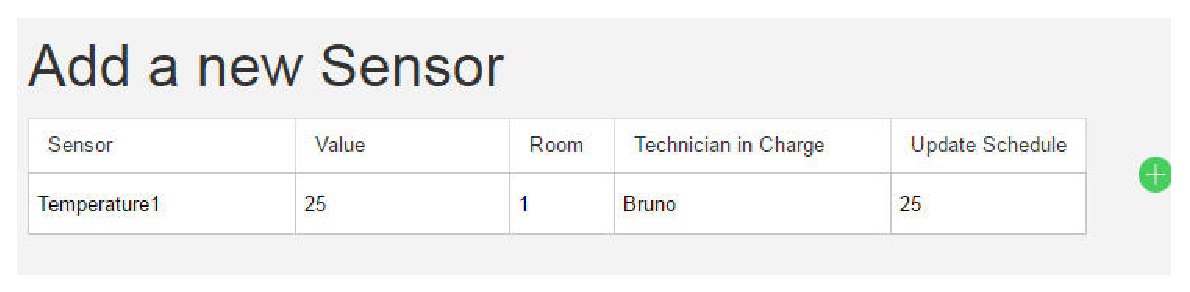
\includegraphics[width=1\textwidth]{images/AddANewSensorTechnician.eps}
\end{figure}
\item System pushes now the information to the sensor table and updates it by
adding the sensor with the other informations added.
\end{enumerate}
\end{description}

\subsubsection{Example of adding a new sensor}
\textbf{Technician} complets the given input text fields with the sensor name
:Temperature1 value 32 degrees and the room: 1 technician name :Bruno and the
update schedule is 15. \textbf{System} pushes the information to the sensor
table and displays the new updated table.
\hfill
\vspace{0.5cm}
\hrule


\break
\subsection{Remove  requested sensor}

\hrule
\hfill
\vspace{0.5cm}
\label{operation:Remove a new sensor}

The Technician can remove the requested sensor from the request table.
\begin{description}
\item \textbf{Parameters:} /
\item \textbf{Precondition:} The system is bootedup and the technician has to be
logged in and be on the technician screen and a request should be in the
request sensor table.
\item \textbf{Post-condition:} Removes the requested sensor from the sensor
request table.
\item \textbf{Output messages:} Successfully deleted the requested sensor.
\item \textbf{Triggering:}
\begin{enumerate}
\item \textbf{Technician} presses the red button on request sensor table.
\begin{figure}[H]
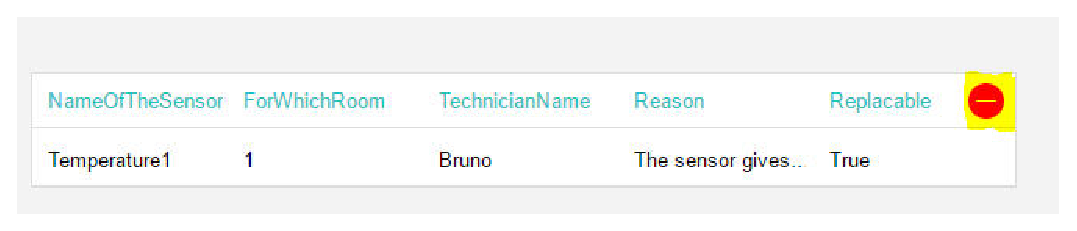
\includegraphics[width=1\textwidth]{images/RemoveSensorFromSensorRequestListTechnician.eps}
\end{figure}
\item System removes sensor from the request table.
\end{enumerate}
\end{description}

\subsubsection{Example of a removing of a sensor}
\textbf{Technician} presses the red button on the ligne 1 of the table where
temperature1 and which room = 1. The system removes the sensor from the request
list.

\hfill
\vspace{0.5cm}
\hrule



\subsection{Filter by sensor type}

\hrule
\hfill
\vspace{0.5cm}

\label{operation:filterSensorTable}

The \textbf{Technician} can filter the table by filter type.
\begin{description}

\item \textbf{Parameters:} /
\item \textbf{Precondition:} The system is bootedup and Technician has to be
logged in and be on the technician screen.
\item \textbf{Post-condition:} The table on the screens show only the filtered
values.
\item \textbf{Output messages:} none
\item \textbf{Triggering:}
\begin{enumerate}
\item \textbf{Technician} choses on the top down menu a sensor type.
\begin{figure}[H]
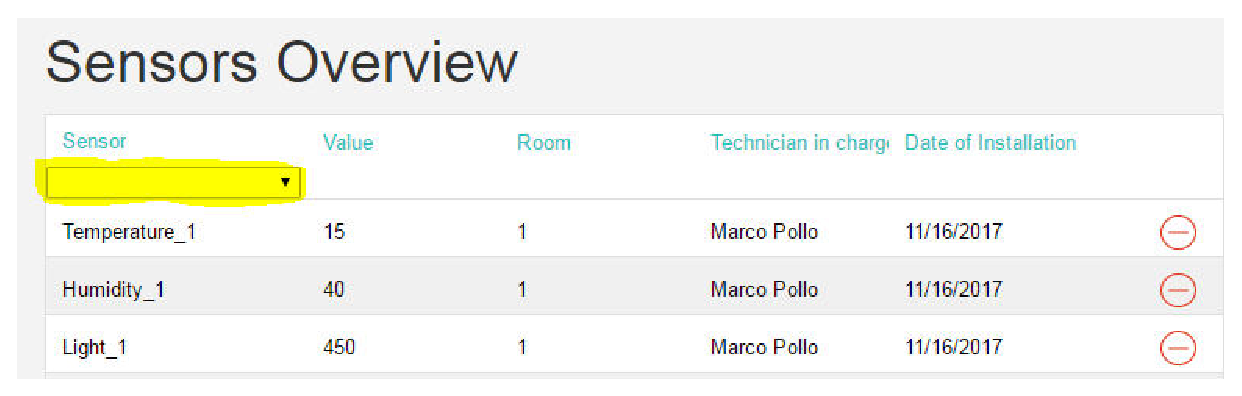
\includegraphics[width=1\textwidth]{images/FilterSensorByTypeTechnician.eps}
\end{figure}
\item System filters out all the non equal types and doesn't display them.
\end{enumerate}
\end{description}

\subsubsection{Example of filtering the Sensors}
\textbf{Technician} choses a type on a the top down menu Temperature. System
know doesn't display the sensor where the type isn't equal to Temperature.
\hfill
\vspace{0.5cm}
\hrule

\break

\subsection{Removes sensor from Sensor Array}

\hrule
\hfill
\vspace{0.5cm}

\label{operation:removesSensor}

The \textbf{Technician} removes the a specific sensor from the table.
\begin{description}

\item \textbf{Parameters:} /
\item \textbf{Precondition:} The system is bootedup and Technician has to be
logged in and be on the technician screen.
\item \textbf{Post-condition:} The table of sensors has been updated on the
technician and gardener screen.
\item \textbf{Output messages:} none
\item \textbf{Triggering:}
\begin{enumerate}
\item \textbf{Technician} choses the sensor which he wants to delete and presses
the red button.
\begin{figure}[H]
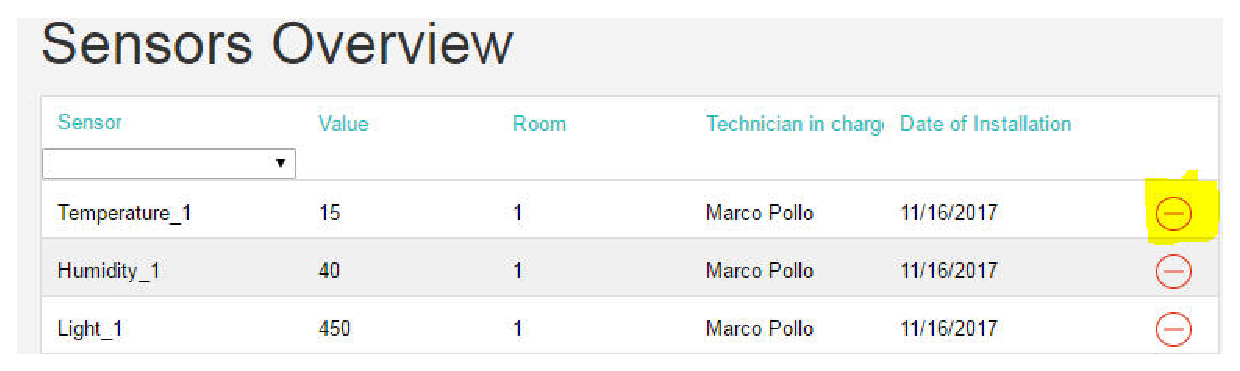
\includegraphics[width=1\textwidth]{images/RemoveSensorFromSensorListTechnician.eps}
\end{figure}
\item System removes the sensor from the table.
\end{enumerate}
\end{description}

\subsubsection{Example of removing Sensor}
\textbf{Technician} choses a given sensors on the Sensor table Temperature 1
sensor and presses the red button on the same line.
System removes the line from the table and reloads the screen to update it.

 \hfill
\vspace{0.5cm}
\hrule